\documentclass[12pt]{article}
\usepackage[english]{babel}
\usepackage[utf8]{inputenc}
\usepackage{amsmath, amssymb,amsthm}
\usepackage{graphicx}
\usepackage{geometry}
\usepackage{hyperref}
\usepackage{xcolor}
\hypersetup{
    colorlinks=true,
    urlcolor=blue
}
\urlstyle{same}
\graphicspath{{./images/}}
\setlength{\topmargin}{0pt}
\setlength{\headsep}{0pt}
\textheight = 600pt

\title{Probability Theory \\ Homework 8}
\author{Ben Kallus}
\date{Due Saturday, November 14}

\begin{document}
\pagecolor{black}
\color{white}
\maketitle

\noindent{\bf 1.}
\begin{align*}
    \mathbb V[Q + R] &= \mathbb E[(Q + R)^2] - \mathbb E[Q + R]^2 \\
                     &= \mathbb E[Q^2 + 2QR + R^2] - (\mathbb E[Q] + \mathbb E[R])^2 \\
                     &= \mathbb E[Q^2] + 2\mathbb E[QR] + \mathbb E[R^2] - \mathbb E[Q]^2 - 2\mathbb E[Q]\mathbb E[R] - \mathbb E[R]^2 \\
                     &= (\mathbb E[Q^2] - \mathbb E[Q]^2) + (\mathbb E[R^2] - \mathbb E[R]^2) + 2(\mathbb E[QR] - \mathbb E[Q]\mathbb E[R]) \\
                     &= \mathbb V[Q] + \mathbb V[R] + 2\text{Cov}(Q,R)
\end{align*}

\newpage
\noindent{\bf 2.} Let $X$ be a random variable with variance $\mathbb V[X] = \sigma^2$ and define $Y = -X$ and $Z = 2X$.

\medskip
\noindent{\bf a.}
\begin{align*}
    \text{Cov}(X,Y) &= \mathbb E[XY] -(\mathbb E[X])(\mathbb E[Y]) \\
                    &= \mathbb E[(X)(-X)] -(\mathbb E[X])(\mathbb E[-X]) \\
                    &= \mathbb -E[X^2] +\mathbb E[X]^2 \\
                    &= \mathbb E[X]^2 - \mathbb E[X^2] \\
                    &= -(\mathbb E[X^2] - \mathbb E[X]^2) \\
                    &= -\sigma^2
\end{align*}
\begin{align*}
    \rho(X,Y) &= \frac{\text{Cov}(X,Y)}{\sqrt{\mathbb V[X]}\sqrt{\mathbb V[Y]}} \\
              &= \frac{-\sigma^2}{\sqrt{\sigma^2} \cdot \sqrt{\sigma^2}} \\
              &= -1
\end{align*}

\medskip
\noindent{\bf b.}
\begin{align*}
    \text{Cov}(X,Z) &= \mathbb E[XZ] -(\mathbb E[X])(\mathbb E[Z]) \\
                    &= 2\mathbb E[X^2] - 2(\mathbb E[X])(\mathbb E[X]) \\
                    &= 2(\mathbb E[X^2] - \mathbb E[X]^2) \\
                    &= 2\sigma^2
\end{align*}
\begin{align*}
    \rho(X,Z) &= \frac{\text{Cov}(X,Z)}{\sqrt{\mathbb V[X]}\sqrt{\mathbb V[Z]}} \\
              &= \frac{2\sigma^2}{\sqrt{\sigma^2} \cdot \sqrt{4\sigma^2}} \\
              &= 1
\end{align*}

\newpage
\noindent{\bf c.}
\begin{align*}
    \text{Cov}(X,3) &= \mathbb E[3X] -(\mathbb E[X])(\mathbb E[3]) \\
                    &= 3\mathbb E[X] - 3\mathbb E[X] \\
                    &= 0
\end{align*}
\begin{align*}
    \rho(X,3) &= \frac{\text{Cov}(X,3)}{\sqrt{\mathbb V[X]}\sqrt{\mathbb V[3]}} \\
              &= \frac{0}{\sqrt{\sigma^2}\sqrt{0}} \\
              &= \frac00 \\
              &= \text{Undefined}
\end{align*}

\newpage
\noindent{\bf 3.}

\medskip
\noindent{\bf a.} $\hat{p_1} = \frac Xn$.
\begin{align*}
    \text{MSE}(\hat{p_1}) &= \text{MSE}\left(\frac Xn\right) \\
                          &= \mathbb V\left[\frac Xn\right] + \left(\text{Bias}\left(\frac Xn\right)\right)^2 \\
                          &= \frac{\mathbb V[X]}{n^2} + \left(\text{Bias}\left(\frac Xn\right)\right)^2 \\
                          &= \frac{\mathbb V[X]}{n^2} + \left( \mathbb E\left[\frac Xn\right] - p \right)^2 \\
                          &= \frac{\mathbb V[X]}{n^2} + \left( \frac{\mathbb E[X]}{n} - p \right)^2 \\
                          &= \frac{np(1-p)}{n^2} + \left( \frac{np}{n} - p \right)^2 \\
                          &= \frac{np(1-p)}{n^2} + \left( p - p \right)^2 \\
                          &= \frac{np(1-p)}{n^2} \\
                          &= \frac{p(1-p)}{n}
\end{align*}

\newpage
\noindent{\bf b.} $\hat{p_2} = \frac{X+1}{n+2}$.
\begin{align*}
    \text{MSE}(\hat{p_2}) &= \text{MSE}\left(\frac{X+1}{n+2}\right) \\
                          &= \mathbb V\left[\frac{X+1}{n+2}\right] + \left(\text{Bias}\left(\frac{X+1}{n+2}\right)\right)^2 \\
                          &= \frac{\mathbb V[X]}{(n+2)^2} + \left(\text{Bias}\left(\frac{X+1}{n+2}\right)\right)^2 \\
                          &= \frac{\mathbb V[X]}{(n+2)^2} + \left( \mathbb E \left[ \frac{X+1}{n+2} \right] - p \right)^2 \\
                          &= \frac{\mathbb V[X]}{(n+2)^2} + \left( \frac{\mathbb E[X+1]}{n+2} - p \right)^2 \\
                          &= \frac{\mathbb V[X]}{(n+2)^2} + \left( \frac{\mathbb E[X] + 1}{n+2} - p \right)^2 \\
                          &= \frac{np(1-p)}{(n+2)^2} + \left( \frac{np + 1}{n+2} - p \right)^2 \\
                          &= \frac{np(1-p)}{(n+2)^2} + \left( \frac{np + 1}{n+2} - \frac{p(n+2)}{n+2} \right)^2 \\
                          &= \frac{np(1-p)}{(n+2)^2} + \left( \frac{np + 1 - p(n+2)}{n+2} \right)^2 \\
                          &= \frac{np(1-p)}{(n+2)^2} + \left( \frac{np + 1 - np-2p}{n+2} \right)^2 \\
                          &= \frac{np(1-p)}{(n+2)^2} + \frac{(-2p + 1)^2}{(n+2)^2} \\
                          &= \frac{np-np^2 + 4p^2 - 4p + 1}{(n+2)^2} \\
                          &= \frac{p^2(4-n)+p(n-4)+1}{(n+2)^2} \\
                          &= \frac{(p - p^2)(n-4)+1}{(n+2)^2}
\end{align*}

\newpage
\noindent{\bf c.} $\hat{p_3} = \frac12$.
\begin{align*}
    \text{MSE}(\hat{p_3}) &= \text{MSE}\left(\frac12\right) \\
                          &= \mathbb V\left[\frac12\right] + \left(\text{Bias}\left(\frac12\right)\right)^2 \\
                          &= \left(\text{Bias}\left(\frac12\right)\right)^2 \\
                          &= \left(\frac12 - p\right)^2 \\
                          &= p^2 - p + \frac14
\end{align*}

\newpage
\noindent{\bf 4.} $\hat p_1$ and $\hat p_2$ are consistent for all possible values of $p$. This is because for each of these two estimators, the limit a $n \to \infty$ of its MSE is 0. Thus, as $n$ gets arbitrarily large, it becomes an arbitrarily good approximation for $p$.

\newpage
\noindent{\bf 5.}

\medskip
\noindent{\bf a.}
\begin{align*}
    \mathbb E[X] &= \overline X \\
    \frac1\lambda &= \overline X \\
    \lambda &= \frac{1}{\overline X}
\end{align*} Thus, \[\hat{\lambda}_{\text{MoM}} = \frac1{\overline X}.\]

\newpage
\noindent{\bf b.}
\begin{align*}
    \mathcal L(\lambda) &= f_X(X_1) \cdot f_X(X_2) \cdot \hdots \cdot f_X(x_n) \\
                        &= \prod_{i=1}^n f_X(X_i) \\
                        &= \prod_{i=1}^n \lambda e^{-\lambda X_i}.
\end{align*} Maximizing this expression is equivalent to maximizing
\begin{align*}
    \ln\left(\prod_{i=1}^n \lambda e^{-\lambda X_i}\right) &= \sum_{i=1}^n \ln\left(\lambda e^{-\lambda X_i}\right) \\
                                                           &= \sum_{i=1}^n \ln(\lambda) + \ln\left(e^{-\lambda X_i}\right) \\
                                                           &= n\ln(\lambda) + \sum_{i=1}^n -\lambda X_i \\
                                                           &= n\ln(\lambda) - \lambda \sum_{i=1}^n X_i.
\end{align*}
Setting the derivative equal to 0, we get
\begin{align*}
    \frac n\lambda - \sum_{i=1}^n X_i &= 0 \\
    \frac n\lambda &= \sum_{i=1}^n X_i \\
    \lambda &= \frac n{\sum\limits_{i=1}^n X_i} \\
            &= \frac 1{\overline X}
\end{align*} Thus, \[\hat\lambda_{MLE} = \frac1{\overline X}.\]

\newpage
\noindent{\bf 6.}

\medskip
\noindent{\bf a.}
\begin{align*}
    \mathbb E[X] &= \frac1n\sum_{i=1}^n X_i \\
    \frac{\alpha + \beta}2 &= \frac1n\sum_{i=1}^n X_i \\
    \alpha + \beta &= 2\overline X \\
    \beta &= 2\overline X - \alpha
\end{align*}
\begin{align*}
    \mathbb E[X^2] &= \overline{X^2} \\
    \mathbb V[X] + \mathbb E[X]^2 &= \overline{X^2} \\
    \frac{(\alpha - \beta)^2}{12} + \frac{(\alpha + \beta)^2}{2^2} &= \overline{X^2} \\
    \frac{(\alpha - \beta)^2 + 3(\alpha + \beta)^2}{12} &= \overline{X^2} \\
    \frac{\alpha^2 -2\alpha\beta + \beta^2 + 3(\alpha^2 + 2\alpha\beta + \beta^2)}{12} &= \overline{X^2} \\
    \frac{4\alpha^2 + 4\alpha\beta + 4\beta^2}{12} &= \overline{X^2} \\
    \alpha^2 + \alpha(2\overline X - \alpha) + (2\overline X - \alpha)^2 &= 3\overline{X^2} \\
    \alpha^2 + 2\alpha\overline X - \alpha^2 + 4\overline X^2 + \alpha^2 - 4\alpha\overline X &= 3\overline{X^2} \\
    \alpha^2 - 2\alpha\overline X + 4\overline X^2 - 3\overline{X^2} &= 0 \\
\end{align*} Thus, by the quadratic formula,
\begin{align*}
    \alpha &= \overline{X} \pm \sqrt3 \sqrt{\overline{X^2} - \overline{X}^2}
\end{align*} $\alpha$ is not equal to $\overline{X} + \sqrt3 \sqrt{\overline{X^2} - \overline{X}^2}$ because if it were, then $\beta$ would be $2\overline X - \overline{X} - \sqrt3 \sqrt{\overline{X^2} - \overline{X}^2}$, which would make $\beta < \alpha$.

Thus,
\begin{align*}
    \alpha &= \overline{X} - \sqrt3 \sqrt{\overline{X^2} - \overline{X}^2} \\
    \beta &= \overline{X} + \sqrt3 \sqrt{\overline{X^2} - \overline{X}^2}
\end{align*}

\newpage
\noindent{\bf b.}
\begin{align*}
    \mathcal L(\alpha, \beta) &= \prod_{i=1}^n f_X(X_i) \\
                              &= \prod_{i=1}^n \frac1{\beta - \alpha} \\
                              &= \frac1{(\beta - \alpha)^n}
\end{align*} At this point, we'd normally maximize the log, but I think in this case we don't even need to. To maximize this expression, we should minimize the denominator, which means we should minimize $\beta$ and maximize $\alpha$. All the sample points have to be between $\alpha$ and $\beta$, so we should choose $\beta = \max\{X_i~|~1 \leq i \leq n\}$, and $\alpha = \min\{X_i~|~1 \leq i \leq n\}$.

\medskip
\noindent{\bf c.} I think the MLE makes more sense because the MoM involves irrational square roots, and it seems unlikely to me that a coin would have an irrational probability of heads.

\newpage
\noindent{\bf 7.} Double eggs.
\begin{center}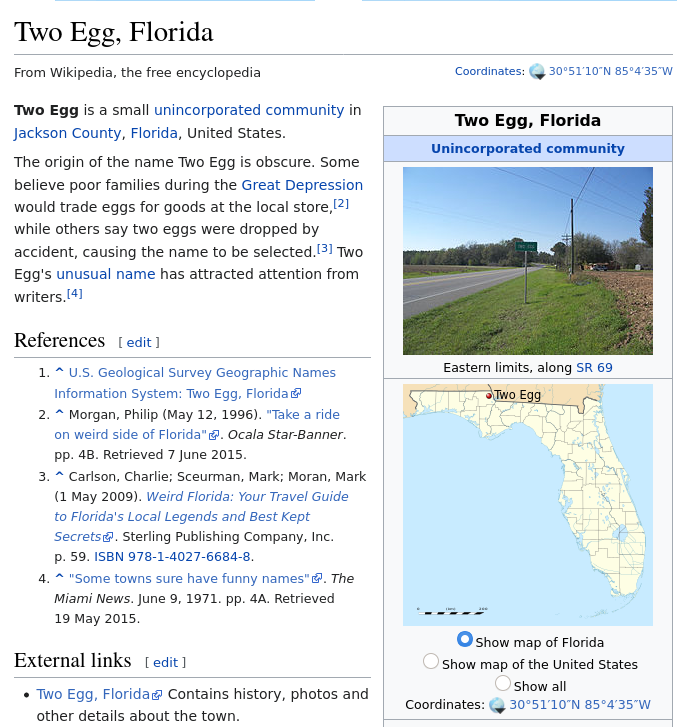
\includegraphics{two-egg.png}\end{center}

\end{document}
